%%%
\documentclass[mathserif, aspectratio=43]{beamer}

\usetheme{metropolis}

\metroset{progressbar=frametitle}

\usefonttheme{professionalfonts}
\usepackage{mathtools}
\usepackage{mathspec}

\makeatletter % undo the wrong changes made by mathspec
\let\RequirePackage\original@RequirePackage
\let\usepackage\RequirePackage
\makeatother

\setmathfont{Latin Modern Math}
\usepackage[none]{hyphenat}

%%% Packages section %%%
\usepackage{hyperref}
\usepackage{amsmath}
\usepackage{amsfonts}
\usepackage{tikz}
\usepackage{minted}

%%% Preamble %%%
\title{Machine Learning and Data Mining}
\subtitle{Recapitulation}
\author{Maxim Borisyak}

\institute{National Research University Higher School of Economics (HSE)}

\usepackage{algorithm}
\usepackage{algpseudocode}
\usepackage{setspace}
\usepackage{framed}

\DeclareMathOperator*{\E}{\mathbb{E}}

\DeclareMathOperator*{\var}{\mathbb{D}}
\newcommand\D[1]{\var\left[ #1 \right]}

\newcommand\dmid{\,\|\,}

\DeclareMathOperator*{\argmin}{\mathrm{arg\,min}}
\DeclareMathOperator*{\argmax}{\mathrm{arg\,max}}


\begin{document}

\begin{frame}[plain]
	\titlepage
\end{frame}

\section{Statistical estimations}



\begin{frame}[fragile]
\frametitle{Setup}
Given:
\begin{itemize}
\item data: $X = \{ x_i \}^N_{i = 1}$;
\item parameterized family of distributions $P(x \mid \theta)$.
\end{itemize}
Problem:
\begin{itemize}
\item estimate $\theta$.
\end{itemize}

\end{frame}


\begin{frame}[fragile]
\frametitle{Maximum likelihood estimation}
\begin{eqnarray*}
L(\theta) &=& P(X \mid \theta);\\
\hat{\theta} &=& \argmax_\theta L(\theta).
\end{eqnarray*}
\begin{equation*}
\mathcal{L}(\theta) = -\log \prod_i P(x_i \mid \theta) = -\sum_i \log P(x_i \mid \theta)
\end{equation*}
\begin{itemize}
\item consistent estimation: $\hat{\theta} \to \theta$ as $N \to \infty$;
\item \textit{might be biased};
\item equal to MAP estimation with uniform prior.
\end{itemize}

\end{frame}


\begin{frame}[fragile]
\frametitle{MLE: example}
\begin{quote}
Given samples $\{ x_i \}^N_{i = 1}$ from a normal distribution estimate its mean.

\end{quote}
\begin{multline*}
  \mu = \argmin_\mu \mathcal{L}(X) = \\[3mm]
    \argmin_mu -\sum_i \log \left(\frac{1}{Z} \exp\left[ -\frac{(x_i - \mu) ^ 2}{2 \sigma^2}\right]\right) = \\[3mm]
    \argmin_\mu \sum_i (x_i - \mu) ^ 2 = \frac{1}{N} \sum_i x_i
\end{multline*}

\end{frame}


\begin{frame}[fragile]
\frametitle{Bayesian inference}
\begin{equation*}
  P(\theta \mid X) = \frac{1}{Z} P(X \mid \theta) P(\theta);
\end{equation*}
\begin{itemize}
\item often, posterior distribution of predictions is of the main interest:
$$P(f(x) = y \mid X) = \int \mathbb{I}\left[ f(x, \theta) = y \right] P(\theta \mid X)\;d\theta$$
\item with a few exceptions posterior is intractable;
\item often, approximate inference is utilized instead.
\end{itemize}

\end{frame}


\begin{frame}[fragile]
\frametitle{BI: example}
\begin{quote}
Given samples $\{x_i\}^N_{i = 1}$ from a normal distribution estimate mean under a normal prior.

\end{quote}
\begin{multline*}
  P(\mu \mid X) = \frac{1}{Z} P(X \mid \mu) P(\mu) = \\
    \frac{1}{Z} \exp\left[ -\frac{\mu ^ 2}{2 c^2}\right] \cdot \prod \exp\left[ -\frac{(x_i - \mu) ^ 2}{2 \sigma^2}\right]
\end{multline*}
\vspace*{5mm}
\begin{equation*}
  \log P(\mu \mid X) = -Z -\frac{\mu ^ 2}{2 c^2} -\sum_i \frac{(x_i - \mu) ^ 2}{2 \sigma^2}
\end{equation*}

\end{frame}


\begin{frame}[fragile]
\frametitle{Maximum a posteriori estimation}
\begin{multline*}
  \hat{\theta} = \argmax_\theta P(\theta \mid X) =
    \argmax_\theta P(X \mid \theta) P(\theta) =\\
    \argmin_\theta \left[  -\log P(X \mid \theta) - \log P(\theta) \right] = \\
    \argmin_\theta \left[  \mathrm{neg\;log\;likelihood} + \mathrm{penalty} \right]
\end{multline*}
\begin{equation*}
\hat{\theta} = \argmin_\theta \left[ -\log P(\theta) - \sum_i \log P(x_i \mid \theta)\right]
\end{equation*}
\begin{itemize}
\item sometimes called \textbf{structural loss}:\begin{itemize}
\item i.e. includes 'structure' of the predictor into the loss.
\end{itemize}

\end{itemize}

\end{frame}


\begin{frame}[fragile]
\frametitle{MAP: example}
\begin{quote}
Given samples $\{x_i\}^N_{i = 1}$ from a normal distribution estimate mean under a normal prior.

\end{quote}
\begin{multline*}
  \hat{\mu} = \argmax_\mu \log P(\mu \mid X) = \\
    \argmax_\mu \left[ -Z -\frac{\mu ^ 2}{2 c^2} - \sum_i \frac{(x_i - \mu) ^ 2}{2 \sigma^2} \right] = \\
    \argmin_\mu \left[ \lambda \mu ^ 2 + \sum_i (x_i - \mu) ^ 2 \right] =
    \frac{1}{N + \lambda} \sum_i x_i
\end{multline*}

\end{frame}


\section{Machine Learning}



\begin{frame}[fragile]
\frametitle{Structure of a Machine Learning problem}
Given:
\begin{itemize}
\item description of the problem:\begin{itemize}
\item prior knowledge;
\end{itemize}

\item data:\begin{itemize}
\item input space: $\mathcal{X}$;
\item output space: $\mathcal{Y}$;
\end{itemize}

\item metric $M$.
\end{itemize}
Problem:
\begin{itemize}
\item find a learning algorithm: $A: \mathcal{D} \to (\mathcal{X} \to \mathcal{Y})$ such that:
$$M(A(\mathrm{data})) \to \max$$
\end{itemize}

\end{frame}


\begin{frame}[fragile]
\frametitle{Differences from statistics}
Machine Learning:
\begin{itemize}
\item usually, probability densities are intractable;
\item high-dimensionality/small sample sizes;
\item hence, no p-values etc;
\item less formal assumptions.
\end{itemize}

\end{frame}


\section{Supervised learning}



\begin{frame}[fragile]
\frametitle{Regression}
Output: $y \in \mathbb{R}$.
\\[5mm]
Assumptions:
\begin{itemize}
\item $y = f(x) + \varepsilon(x)$;
\item $\varepsilon(x)$ - noise:
\begin{itemize}
\item $\forall x_1, x_2: x_1 \neq x_2 \Rightarrow \varepsilon(x_1)\;\text{independent from}\; \varepsilon(x_2)$;
\item $\forall x: \E \varepsilon(x) = 0$.
\end{itemize}

\item often, $\varepsilon(x)$ is assumed not to be dependent on $x$.

\end{itemize}

\end{frame}


\begin{frame}[fragile]
\frametitle{Regression loss}
\begin{multline*}
  \mathcal{L}(f) = -\sum_i \log P((x_i, y_i) \mid f) = \\
    -\sum_i \log P_\varepsilon(y_i - f(x_i) \mid f, x_i) =\\
    -\sum_i \log P_\varepsilon(y_i - f(x_i) \mid x_i)
\end{multline*}

\end{frame}


\begin{frame}[fragile]
\frametitle{Regression: MSE}
\begin{itemize}
\item $\varepsilon \sim \mathcal{N}(0, \sigma^2_\varepsilon)$;
\item $\sigma^2_\varepsilon = \mathrm{const}$ (unknown);
\end{itemize}
\begin{multline*}
  \mathcal{L}(f) = -\sum_i \log P_\varepsilon(y_i - f(x_i) \mid x_i) = \\
    \sum_i \left[ Z(\sigma^2_\varepsilon) - \frac{(y_i - f(x_i))^2}{2 \sigma^2_\varepsilon}\right] \sim \\
    \sum_i (y_i - f(x_i))^2 \to \min
\end{multline*}
\begin{equation*}
  f^*(x) = \E\left[ y \mid x \right]
\end{equation*}

\end{frame}


\begin{frame}[fragile]
\frametitle{Regression: MAE}
\begin{itemize}
\item $\varepsilon \sim \mathrm{Laplace}(0, b_\varepsilon)$;
\item $b_\varepsilon = \mathrm{const}$ (unknown);
\end{itemize}
\begin{multline*}
  \mathcal{L}(f) = -\sum_i \log P_\varepsilon(y_i - f(x_i) \mid x_i) = \\
    \sum_i \left[ Z(b_\varepsilon) - \frac{|y_i - f(x_i)|}{2 b_\varepsilon}\right] \sim \\
    \sum_i |y_i - f(x_i)| \to \min
\end{multline*}
\begin{equation*}
  f^*(x) = \mathrm{median}\left[ y \mid x \right]
\end{equation*}

\end{frame}


\begin{frame}[fragile]
\frametitle{Linear regression}
$$f(x) = w \cdot x$$

\footnotetext[1]{For clarity we omit the bias term as it can be included by appending 1 to every sample.}

\end{frame}


\begin{frame}[fragile]
\frametitle{Linear regression + MSE + MLE}
\begin{eqnarray*}
  \mathcal{L}(w) &=& \sum_i (w \cdot x_i - y_i) ^ 2 = \|X w - y\|^2 \to \min;\\
  \frac{\partial}{\partial w}\mathcal{L}(w) &=& 2 X^T (X w - y) = 0;\\
  w &=& (X^T X)^{-1} X^T y.
\end{eqnarray*}

\end{frame}


\begin{frame}[fragile]
\frametitle{Linear regression + MSE + MAP}
\begin{eqnarray*}
  \mathcal{L}(w) &=& \sum_i (w \cdot x_i - y_i) ^ 2 + \lambda \|w\|^2 =\\
    && \|X w - y\|^2 + \lambda \|w\|^2\to \min;\\
  \frac{\partial}{\partial w}\mathcal{L}(w) &=& 2 X^T (X w - y) + 2 \lambda w= 0;\\
  w &=& (X^T X + \lambda I)^{-1} X^T y.
\end{eqnarray*}

\end{frame}


\begin{frame}[fragile]
\frametitle{Linear regression + MSE + Bayesian Inference}
\begin{itemize}
\item prior:
$$w \sim \mathcal{N}(0, \Sigma_w);$$
\item data model:
$$\varepsilon \sim \mathcal{N}(0, \sigma^2_\varepsilon).$$
\end{itemize}

\end{frame}


\begin{frame}[fragile]
\frametitle{Linear regression + MSE + Bayesian Inference}
\begin{multline*}
P(w \mid y, X) \propto P(y \mid w, X) P(w) \propto \\[3mm]
  \exp\left[ - \frac{1}{2 \sigma^2_\varepsilon} (y - X w)^T (y - X w) \right] \cdot \exp\left[ -\frac{1}{2} w^T \Sigma^{-1}_w w \right] = \\[3mm]
  \exp\left[ - \frac{1}{2} (w - w^*)^T A_w (w - w^*) \right]
\end{multline*}
where:
\begin{itemize}
\item $A_w = \frac{1}{\sigma^{2}_\varepsilon}X X^T + \Sigma^{-1}_w$;
\item $w^* = \frac{1}{\sigma^{2}_\varepsilon} A^{-1}_w X y$.
\end{itemize}

\end{frame}


\begin{frame}[fragile]
\frametitle{Linear regression + MSE + Bayesian Inference}
To make prediction $y'$ in point $x'$:
\begin{multline*}
P(y' \mid y, X, x') = \\
  \int P(y' \mid w, x') P(w \mid X, y) = \\
  \mathcal{N}\left( \frac{1}{\sigma^2_\varepsilon} x'^T A^{-1} X y, x'^T A^{-1} x' \right)
\end{multline*}

\end{frame}


\begin{frame}[fragile]
\frametitle{Basis expansion}
To capture more complex dependencies basis functions can be introduced:
$$f(x) = \sum_i w \cdot \phi(x)$$

where:
\begin{itemize}
\item $\phi(x) \in \mathbb{R}^K$ - expanded basis.
\item $\phi$ \textbf{is fixed}.
\end{itemize}

\end{frame}


\begin{frame}[fragile]
\frametitle{Basis expansion: example}
Regression with polynomials:
$$\phi(x) = \{1, x_1, \dots, x_n, x^2_1, x_1 x_2, \dots, x^2_n, \dots\}$$

Periodic functions:
$$\phi(x) = \{1, \sin(x), \cos(x), \sin(2x), \cos(2x), \dots\}$$


\end{frame}


\begin{frame}[fragile]
\frametitle{Basis expansion: example}
\begin{figure}
\centering
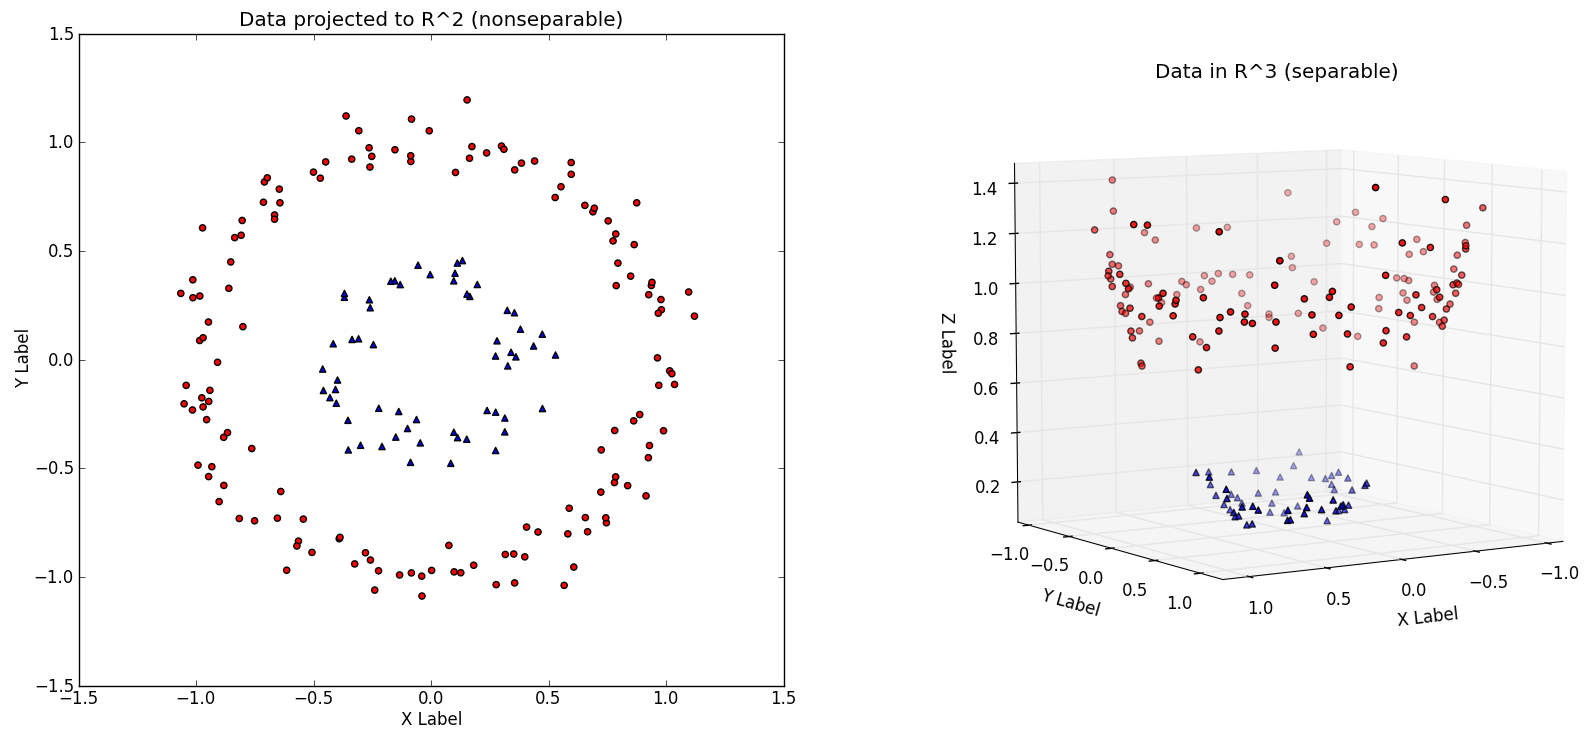
\includegraphics[width=1\textwidth]{/tmp/tmpdk09w3m9mdslides/mdslides/kernel-trick.png}

\end{figure}

{
  \footnotesize
  Source: \texttt{eric-kim.net}
}

\end{frame}


\begin{frame}[fragile]
\frametitle{Classification}
\begin{itemize}
\item classes: $y \in \{1, 2, \dots, m\}$;
\item classifier:
\end{itemize}
\begin{eqnarray*}
  f: \mathcal{X} \to \mathbb{R}^m;\\
  \sum^m_{k=1} f^k(x) = 1.
\end{eqnarray*}
\begin{eqnarray*}
  \mathcal{L}(f) = -\sum_i \sum^m_{k = 1} \mathbb{I}[y_i = k]\log f^k(x_i);\\
  \mathrm{cross\text{-}entopy}(f) = \sum_i y'_i \cdot f(x_i).
\end{eqnarray*}

\end{frame}


\begin{frame}[fragile]
\frametitle{Softmax}
\begin{itemize}
\item often employed trick to make $f(x)$ a proper distribution:
\end{itemize}
\begin{eqnarray*}
f(x) &=& \mathrm{softmax}(g(x));\\[5mm]
f^i(x) &=& \frac{\exp(g^i(x))}{\sum_k \exp(g^k(x))}.
\end{eqnarray*}

\end{frame}


\begin{frame}[fragile]
\frametitle{Logistic regression}
\begin{eqnarray*}
  g(x) &=& W x + b;\\
  f(x) &=& \mathrm{softmax}(g(x)).
\end{eqnarray*}
Another form:
\begin{eqnarray*}
  \frac{\log P(y = i \mid x)}{\log P(y = j \mid x)} = \frac{w_i \cdot x + b_i}{w_j \cdot x + b_j}
\end{eqnarray*}

\end{frame}


\begin{frame}[fragile]
\frametitle{Logistic regression: 2 classes}
\begin{multline*}
  f_1(x) = \frac{\exp(w_1 \cdot x + b_1)}{\exp(w_1 \cdot x + b_1) + \exp(w_2 \cdot x + b_2)} =\\[5mm]
    \frac{1}{1 + \exp((w_2 - w_1) \cdot x + b_2 - b_1)} =\\[5mm]
    \frac{1}{1 + \exp(w' \cdot x + b')} = \\[5mm]
    \mathrm{sigmoid}(w' \cdot x + b').
\end{multline*}

\end{frame}


\begin{frame}[fragile]
\frametitle{Logistic regression: 2 classes}
\begin{figure}
\centering
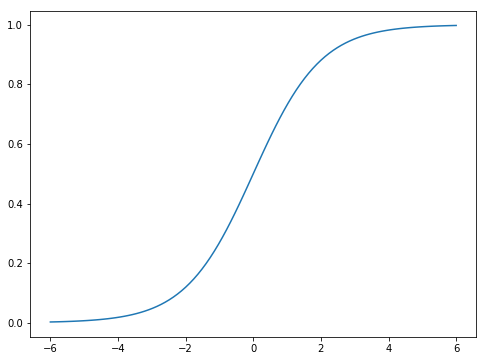
\includegraphics[width=1\textwidth]{/tmp/tmpdk09w3m9mdslides/mdslides/sigmoid.png}

\end{figure}


\end{frame}


\begin{frame}[fragile]
\frametitle{Training logistic regression}
\begin{multline*}
  \mathcal{L}(w) = \\
  \sum_i \mathbb{I}[y_i = 1] \log (1 + \exp(w x_i + b)) + \mathbb{I}[y_i = 0] \log (1 + \exp(-w x_i - b))
\end{multline*}
\begin{itemize}
\item has no analytical solution;
\item smooth and convex.
\end{itemize}

\end{frame}


\begin{frame}[fragile]
\frametitle{Gradient Descent}
\begin{eqnarray*}
f(\theta) \to \min;\\
\theta^* = \argmin_\theta f(\theta).
\end{eqnarray*}
\begin{eqnarray*}
  \theta^{t + 1} &=& \theta^t - \alpha \nabla f(\theta^t);\\
  \theta^t &\to& \theta^*, t \to \infty;\\
\end{eqnarray*}

\end{frame}


\begin{frame}[fragile]
\frametitle{Gradient Descent}
\begin{framed}
\begin{spacing}{1.75}
\begin{algorithmic}[1]
  \State $\theta := \text{initialization}$
  \For{$t := 1, \dots$}
    \State $\theta := \theta - \alpha \nabla f(\theta^t)$
  \EndFor
\end{algorithmic}
\end{spacing}
\end{framed}

\end{frame}


\begin{frame}[fragile]
\frametitle{Stochastic Gradient Descent}
$$f(\theta) = \sum^N_{i = 1} f_i(\theta)$$

\begin{framed}
\begin{spacing}{1.75}
\begin{algorithmic}[1]
  \State $\theta := \text{initialization}$
  \For{$t := 1, \dots$}
    \State $i := \mathrm{random}(1, \dots, N)$
    \State $\theta := \theta - \alpha \nabla f_i(\theta^t)$
  \EndFor
\end{algorithmic}
\end{spacing}
\end{framed}

\end{frame}


\begin{frame}[fragile]
\frametitle{Illustration}
\begin{figure}
\centering
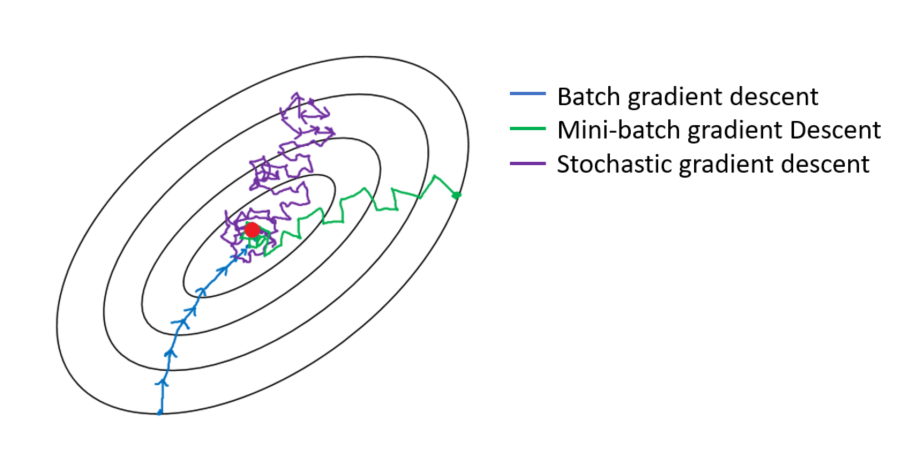
\includegraphics[width=1\textwidth]{/tmp/tmpdk09w3m9mdslides/mdslides/sgd.png}

\end{figure}

{
  \footnotesize
  Source: \texttt{towardsdatascience.com}
}

\end{frame}


\begin{frame}[fragile]
\frametitle{Tricky example}
\begin{figure}
\centering
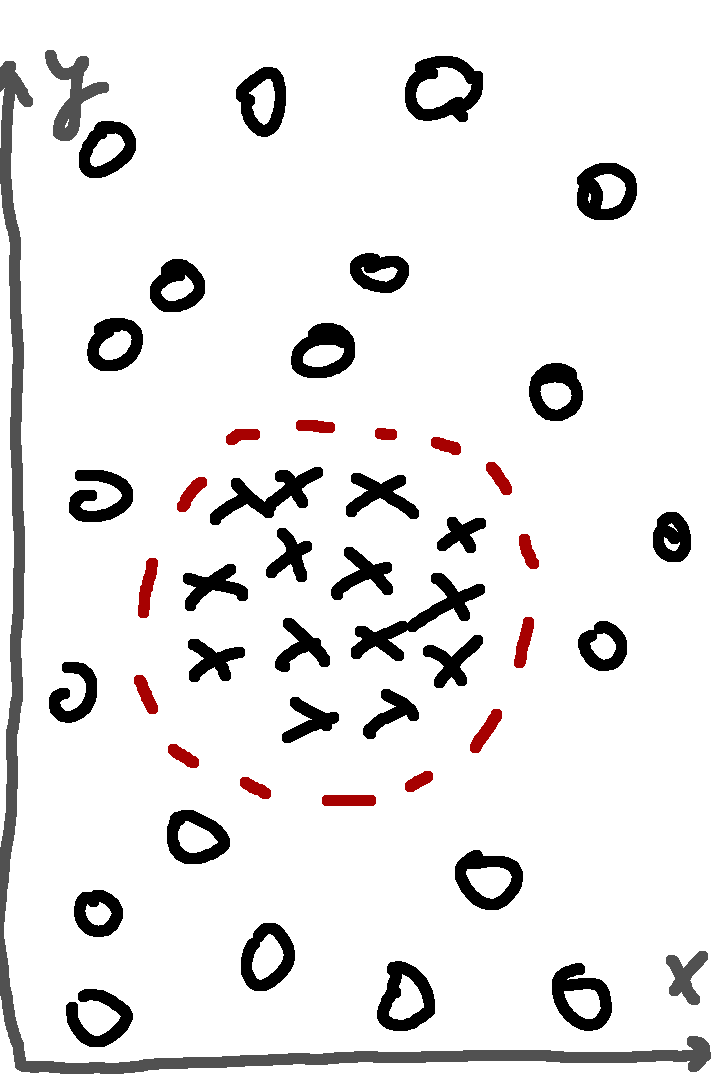
\includegraphics[width=1\textwidth]{/tmp/tmpdk09w3m9mdslides/mdslides/example-1.png}

\end{figure}


\end{frame}


\begin{frame}[fragile]
\frametitle{Tricky example}
\begin{figure}
\centering
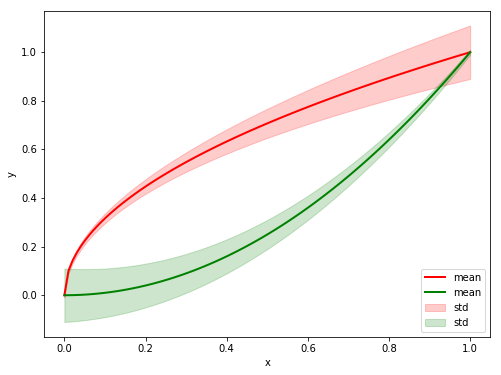
\includegraphics[width=1\textwidth]{/tmp/tmpdk09w3m9mdslides/mdslides/example-2.png}

\end{figure}


\end{frame}


\begin{frame}[fragile]
\frametitle{...}
\begin{figure}
\centering
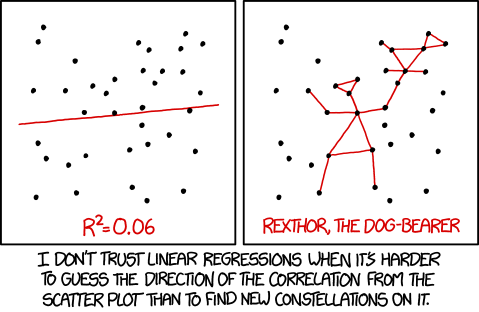
\includegraphics[width=0.9\textwidth]{/tmp/tmpdk09w3m9mdslides/mdslides/xkcd-regression-1.png}

\end{figure}

{
  \footnotesize
  Source: \texttt{xkcd.com}
}

\end{frame}


\section{My first neural network}



\begin{frame}[fragile]
\frametitle{Universal Approximators}
\begin{block}{Universal Approximation Theorem}
  If $\phi$ is a non-constant, continuous, bounded, monotonic function, then every continuous function $f$ on a compact set from $\mathbb{R}^n$
  can be approximated with any precision $\varepsilon > 0$ by:
    $$g(x) = c + \sum^N_{i = 1} \alpha_i \phi(w_i \cdot x + b_i)$$
  given large enough $N$.
\end{block}

\end{frame}


\begin{frame}[fragile]
\frametitle{Universal Approximators}
\begin{figure}
\centering
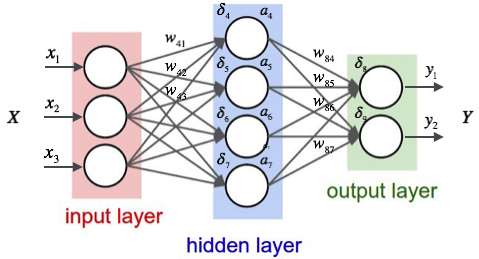
\includegraphics[width=1\textwidth]{/tmp/tmpdk09w3m9mdslides/mdslides/mlp.png}

\end{figure}


\end{frame}


\begin{frame}[fragile]
\frametitle{How to train a neural network}
Stochastic Gradient Descent and Co.

\end{frame}


\begin{frame}[fragile]
\frametitle{How to train a neural network}
Stochastic Gradient Descent and Co.
\begin{itemize}
\item how to initialize?
\item how to choose an appropriate learning rate?
\item how many units?
\item which activation function to choose?
\end{itemize}

\end{frame}

\end{document}
